\documentclass[10pt,a4paper]{article}
\usepackage[margin=2.2cm]{geometry}
\usepackage{fontspec}
\usepackage{kotex}
\setmainfont{Apple SD Gothic Neo}
\setsansfont{Apple SD Gothic Neo}
\usepackage{amsmath,amssymb}
\usepackage{graphicx}
\usepackage{booktabs}
\usepackage{caption}
\usepackage[dvipsnames]{xcolor}
\usepackage[colorlinks=true,linkcolor=MidnightBlue,citecolor=MidnightBlue,
            urlcolor=MidnightBlue]{hyperref}
\usepackage{titlesec}
\titleformat{\section}{\large\bfseries}{\thesection}{0.6em}{}
\titleformat{\subsection}{\normalsize\bfseries}{\thesubsection}{0.5em}{}
\captionsetup{font=small,labelfont=bf}
\setlength{\parskip}{0.35em}
\setlength{\parindent}{0pt}

\usepackage{mdframed}
\newmdenv[linewidth=0.4pt,linecolor=gray!60,backgroundcolor=gray!5,
          innertopmargin=6pt,innerbottommargin=6pt,skipabove=8pt,skipbelow=8pt]{claimbox}
\newcommand{\claim}[2]{\begin{claimbox}\textbf{주장.} #1\par\smallskip
  \textcolor{gray!70}{\textbf{반증 조건.} #2}\end{claimbox}}

\title{\bfseries 가드가 잘못된 시험대에서 왔다\\[2pt]
\large 판에서 쓰레기 열은 열당 $0.0015$ 다 --- 원노트에는 그 값이 있었고 요약이 그것을 떨어뜨렸다}
\author{월드모델 실험실 · 노트 737 · 738}
\date{2026-08-06}
\begin{document}\maketitle

\section{한 줄}

이 실험실의 상시 가드에 \textbf{``열을 적게 넣는다 --- 얇은 도메인에서 열 하나당
$\rho$ $0.02{\sim}0.025$''}가 있다. 그 값을 \textbf{판에서 신호 없는 열로 쟀다.} 순수 난수 열을
넣으니 \textbf{가장 비싼 열이 열당 $0.0015$} 이고 \textbf{연속 쓰레기 세 열이
$0.0043$ --- 판 $2\sigma$($0.0045$)와 같다.} 즉 \textbf{쓰레기 열 셋이 겨우 문턱
하나만큼 깎는다.} 내 사전등록 예측 여덟 개 중 다섯이 \textbf{전부 같은 방향으로}
틀렸다 --- 나는 비용을 $10{\sim}25$배 크게 잡고 있었다.

\section{왜 이 실험이 필요했나 --- 앞의 비교가 교란돼 있었다}

노트 $694$ 가 곁가지로 이런 것을 봤다: 같은 $2$열인데 \textbf{난수 연속은
$-0.0794$}(열당 $0.040$)이고 \textbf{이산 제작사는 $-0.002$}(열당 $0.001$)로
$\mathbf{40}$\textbf{배} 차이다. 그래서 \emph{``차원 비용은 열의 거칠기에
달렸다''}는 가설이 생겼다.

\textbf{그 비교는 셋이 동시에 다르다.}

\begin{center}
\begin{tabular}{ll}
\toprule
① 카디널리티 & 연속 대 이산 \\
② \textbf{신호를 나르나} & 제작사는 라벨과 관계가 있고 난수는 없다 \\
③ 시험대 & \textbf{판이 아니라 $564$짝 스피어만}이었다 \\
\bottomrule
\end{tabular}
\end{center}

\textbf{그래서 신호를 없애고 카디널리티만 남겼다.} 도메인마다 연속 난수 $3$벡터를
뽑고 \textbf{팔마다 그것을 도메인 안 분위로 이산화}했다 --- $k = 2 \cdot 4 \cdot 10
\cdot 100 \cdot$ 연속. \textbf{팔들이 같은 무작위 위에 짝지어진다.} 그리고 시험대를
\textbf{판}으로 옮겼다($11$ 도메인 · 채점 분모 $3{,}369$ · 씨앗 $6$).

\subsection*{이 실험은 위약이 뒤집혀 있다}

\textbf{모든 팔이 위약이다.} 재는 것이 신호가 아니라 \emph{비용}이므로 ``값만 섞은
팔''을 따로 걸 이유가 없다 --- 난수 열의 값을 섞으면 또 난수 열이다. 기준선이
\textbf{없이}이고 모든 팔은 그보다 나쁠 것이 예상된다. \textbf{그러므로 이 논문은
신호 주장을 하지 않는다.}

\subsection*{배선을 먼저 검사했다 --- 통과}

\texttt{\_idol} 은 행 길이가 안 맞으면 열을 \textbf{$0.5$ · 마스크 $0$ 으로 조용히
중립화}한다(노트 $359$). \textbf{중립화되면 ``비용이 없다''와 ``열이 안 붙었다''가
구분되지 않는다.} 그래서 팔마다 도메인별 (관측 · 고유값)을 찍었다 --- \textbf{일곱
팔 전부 $11$ 도메인에 붙었고} 연속 열의 고유값이 행수와 정확히 같다(게임 $482$ ·
도서 $243$ · 만화 $5{,}905$ · 팝업 $89$). \textbf{중립화 없음.}

기준선은 $\mathbf{0.4685}$ 다 --- 챔피언 기록 $0.4689$(씨앗 $12$)와 맞는다.

\begin{figure}[t]\centering
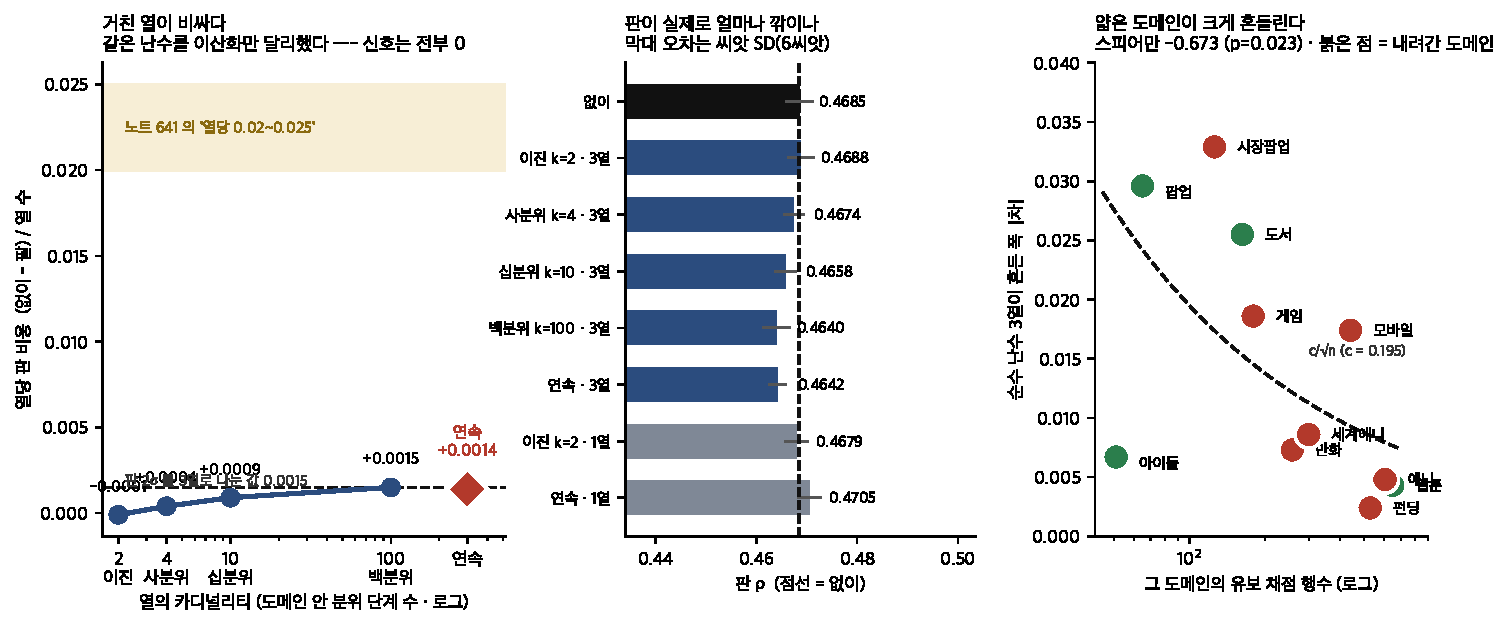
\includegraphics[width=0.99\textwidth]{figs/roughcol.pdf}
\caption{왼쪽: \textbf{거친 열이 비싸지만 폭이 $0.0015$ 다} --- 노란 띠가 내가 써 온
값($0.02{\sim}0.025$)이고 곡선이 그 아래 한참에 있다. 가운데: \textbf{판이 실제로
얼마나 깎이나} --- 막대 오차는 씨앗 SD. 오른쪽: \textbf{얇은 도메인이 크게
흔들린다} --- 순수 난수인데 팝업 · 도서는 오히려 오른다.}
\end{figure}

\section{곡선 --- 방향은 실재하고 크기가 작다}

\begin{center}
\begin{tabular}{lrrrrl}
\toprule
팔 ($3$열) & 판 & 하락 & \textbf{열당} & 짝 $2\sigma$ & 판정 \\
\midrule
없이 & $0.4685$ & --- & --- & --- & 기준선 \\
이진 $k{=}2$ & $0.4688$ & $-0.0003$ & $\mathbf{-0.0001}$ & $0.0035$ & $2\sigma$ 안 \\
사분위 $k{=}4$ & $0.4674$ & $+0.0011$ & $\mathbf{+0.0004}$ & $0.0028$ & $2\sigma$ 안 \\
십분위 $k{=}10$ & $0.4658$ & $+0.0027$ & $\mathbf{+0.0009}$ & $0.0029$ & $2\sigma$ 안 \\
백분위 $k{=}100$ & $0.4640$ & $+0.0045$ & $\mathbf{+0.0015}$ & $0.0034$ & \textbf{$2\sigma$ 밖} \\
연속 & $0.4642$ & $+0.0043$ & $\mathbf{+0.0014}$ & $0.0033$ & \textbf{$2\sigma$ 밖} \\
\midrule
이진 · $1$열 & $0.4679$ & $+0.0006$ & $+0.0006$ & $0.0037$ & $2\sigma$ 안 \\
연속 · $1$열 & $0.4705$ & $\mathbf{-0.0021}$ & $-0.0021$ & $0.0037$ & $2\sigma$ 안 \\
\bottomrule
\end{tabular}
\end{center}

$k{=}2$ 에서 $100$ 까지 \textbf{단조 증가하고 $k \approx 100$ 에서 포화한다} ---
연속이 백분위보다 안 비싸다(차 $0.0001$ 로 잡음 안). \textbf{연속 $-$ 이진 $=
0.0015$/열} 이고 사전등록 문턱 $0.010$ 의 $1/7$ 이다.

씨앗 $6$ 을 \textbf{짝지어} 읽었다(노트 $712$: 씨앗 잡음이 팔에 공통이므로
짝 차의 SD 가 맞는 자다). 거칠기 차도 경계선이다 --- 이진$-$십분위 $+0.0030$
($2\sigma$ $0.0026$ \textbf{밖}) · 이진$-$연속 $+0.0046$($2\sigma$ $0.0045$
간신히 \textbf{밖}) · 이진$-$백분위 $+0.0048$($2\sigma$ $0.0050$ \textbf{안}).

\claim{\textbf{판에서 쓰레기 열 하나는 어느 거칠기에서도 판을 못 움직인다.}
$1$열 팔 둘이 다 $2\sigma$ 안이고 연속 $1$열은 오히려 $-0.0021$(판이 올랐다는
뜻이지만 잡음 안이다). \textbf{$3$열이 되어야 문턱에 닿는다.}}
{$3$열까지만 봤다. \textbf{$10$열 · $30$열에서 볼록해지면 ``열을 적게''가 다시
산다} --- 비용이 열 수에 초선형이면 지금 결론이 ``세 열까지는 싸다''로 좁아진다.
그 측정을 다음 실험으로 등록했다.}

\section{진짜 발견 --- 요약이 시험대를 떨어뜨렸다}

여기서 나는 한 번 더 확인해야 했다. \textbf{노트 $641$ 을 다시 읽으니 판 값이 이미
거기 있었다.}

\begin{center}
\begin{tabular}{llrr}
\toprule
& 출처 & 얇은 도메인(팝업) & \textbf{판} \\
\midrule
방문자 축 $3$열 & 노트 $641$ & $-0.067$ & $\mathbf{-0.0018}$ \\
방문자 축 $1$열 & 노트 $641$ & $+0.009$ & $\mathbf{+0.0008}$ \\
\midrule
쓰레기 연속 $3$열 & \textbf{노트 738} & --- & $\mathbf{-0.0043}$ \\
쓰레기 연속 $1$열 & \textbf{노트 738} & --- & $+0.0021$ \\
\bottomrule
\end{tabular}
\end{center}

\textbf{노트 $641$ 의 판 값($-0.0018$)과 내 실측($-0.0043$)이 같은 자리다.} 즉
\textbf{자료는 처음부터 맞았다.} 그리고 실제 축($-0.0018$)이 쓰레기($-0.0043$)보다
판을 \emph{덜} 깎았다는 것까지 맞는다 --- 그 축이 신호를 얼마간 나른다는 뜻이다.

\textbf{그러면 무엇이 틀렸나. 가드 문장이다.}

\begin{center}
가드에 남은 문장: \emph{``열을 적게 넣는다 --- \textbf{얇은 도메인에서} 열 하나당
$\rho$ $0.02{\sim}0.025$''}\\
\textbf{같이 안 남은 문장}: \emph{``같은 실험의 판 값은 $3$열 $-0.0018$ ·
$1$열 $+0.0008$ 이다''}
\end{center}

\claim{\textbf{요약이 시험대를 떨어뜨렸고, 그 뒤 $96$ 노트 동안 나는 그 요약만
인용했다.} 측정이 틀린 것이 아니라 \textbf{측정을 이고 다니는 문장}이 틀렸다.
그러므로 조항은 ``더 재라''가 아니라 \textbf{``가드를 인용할 때 그 가드가 어느
시험대에서 나왔나를 같이 적는다''}다 --- 규약 $13$(문턱에 $\sigma$ 를 같이 적는다)과
같은 층이고, 층만 다르다: 그쪽은 \emph{잡음의 단위}를 잃고 이쪽은 \emph{시험대}를
잃는다.}
{요약이 값을 하나만 남긴 것이 나쁜 판단이 아니었을 수도 있다 --- 가드는 짧아야
불린다(노트 $598$). \textbf{그렇다면 짧게 유지하면서 시험대를 남기는 방법이
필요하고}, 그것은 ``$0.02{\sim}0.025$''가 아니라 ``\textbf{얇은 도메인} $0.02$ ·
\textbf{판} $0.0015$'' 두 값을 나란히 적는 것이다. 이 논문이 그 두 번째 값을
처음 만들었다.}

\subsection*{그래서 이 논문이 실제로 더한 것}

\begin{center}
\begin{tabular}{ll}
\toprule
① & \textbf{판에서 카디널리티 곡선}(이진 $0$ $\to$ 백분위 $0.0015$ $\to$ 연속 포화) --- 새 값 \\
② & \textbf{$1$열은 어느 거칠기에서도 판을 못 움직인다} --- 노트 $641$ 의 $1$열 $+0.0008$ 을 일반화 \\
③ & \textbf{신호 없는 열로만 쟀다} --- 노트 $641$ 의 방문자 축은 신호가 섞여 있었다 \\
④ & \textbf{도메인 흔들림 $\leftrightarrow$ 유보 행수} 스피어만 $-0.673$ --- 새 값 \\
\bottomrule
\end{tabular}
\end{center}

\subsection*{그래서 변명 하나가 사라졌다}

\textbf{이것은 좋은 소식이 아니다.} 후보 축이 판을 못 움직일 때 나는 \emph{``차원
비용이 이득을 먹었다''}로 읽을 수 있었다. \textbf{판에서 그 비용이 문턱의 $1/3$
이므로 그 설명이 거의 죽는다} --- 남는 설명은 \textbf{신호가 없다}는 것이다.

\claim{\textbf{후보 축이 판을 못 움직이는 이유는 차원 비용이 아니라 신호
없음이다.} 그리고 \textbf{그 반대쪽 함의가 실무적으로 크다} --- 판이 쓰레기 열에
튼튼하므로 \textbf{후보 축을 넓게 탐색해도 된다.} 열 하나를 아끼려고 정보를 버릴
필요가 없었다. \textbf{다만 얇은 도메인에서는 여전히 비싸다}($-0.067$) --- 그래서
``열을 적게''는 \textbf{도메인 결론을 낼 때}는 살아 있고 \textbf{판 결론을 낼 때}만
느슨해진다.}
{쓰레기 열의 \emph{비용}을 쟀고 유용한 열의 \emph{이득}을 잰 것이 아니다. 실제
후보 축은 난수가 아니라 \textbf{라벨과 약하게 상관된} 열이고, 그런 열은 트리가 더
많이 쪼개므로 비용 구조가 다를 수 있다. 그것은 안 쟀다.}

\section{곁가지 --- 시장팝업은 판의 잡음 배수기다}

연속 $3$열이 도메인마다 얼마나 흔드나.

\begin{center}
\begin{tabular}{lrr|lrr}
\toprule
도메인 & 차 & 유보행 & 도메인 & 차 & 유보행 \\
\midrule
\textbf{시장팝업} & $\mathbf{-0.0329}$ & $126$ & 펀딩 & $-0.0024$ & $529$ \\
게임 & $-0.0186$ & $180$ & 웹툰 & $+0.0043$ & $650$ \\
모바일 & $-0.0174$ & $441$ & 아이돌 & $+0.0067$ & $51$ \\
세계애니 & $-0.0086$ & $300$ & 도서 & $+0.0255$ & $163$ \\
만화 & $-0.0073$ & $258$ & \textbf{팝업} & $\mathbf{+0.0296}$ & $65$ \\
애니 & $-0.0048$ & $606$ & & & \\
\bottomrule
\end{tabular}
\end{center}

\textbf{순수 난수인데 팝업과 도서는 오히려 오른다.} $|$흔들림$| \leftrightarrow$
유보 채점 행수 \textbf{스피어만 $-0.673$}($p{=}0.023$) --- \textbf{얇은 도메인이
크게 흔들린다.}

\claim{\textbf{시장팝업의 큰 ``판 기여''는 신호가 아니라 얇음이다.} 그 도메인은
노트 $721$ 에서 신호 몫 $+0.1857$ 을 주고 노트 $729$ 에서 $-0.1191$ 을 줬다 ---
\textbf{부호가 뒤집혔다.} 여기서는 \textbf{순수 난수 $3$열이 그 도메인을 $-0.0329$
흔든다}(도메인 평균의 $7.6$배 · 유보 $126$행). \textbf{세 측정이 한 가지를 말한다
--- 그 도메인은 무엇을 넣어도 크게 움직인다.}}
{$c/\sqrt{n}$ 맞춤은 $c{=}0.195$ 인데 아이돌($51$행 · $|0.0067|$)이 크게 벗어난다.
\textbf{그래서 방향만 말하고 형태는 주장하지 않는다}($n{=}11$). 시장팝업이
$126$행인데 아이돌($51$행)보다 다섯 배 더 흔들리는 것도 설명이 없다 --- 행수 외에
다른 것(라벨 분포의 꼬리?)이 있다.}

\section{사전등록 채점 --- 여덟 중 다섯이 같은 방향으로 틀렸다}

\begin{center}
\begin{tabular}{llll}
\toprule
& 예측 & 실측 & \\
\midrule
① 이진 & $0.002 \sim 0.010$ & $-0.0001$ & \textbf{틀림} \\
② 사분위 & $0.004 \sim 0.014$ & $+0.0004$ & \textbf{틀림} \\
③ 십분위 & $0.010 \sim 0.025$ & $+0.0009$ & \textbf{틀림} \\
④ 백분위 & $0.020 \sim 0.035$ & $+0.0015$ & \textbf{틀림} \\
⑤ 연속 & $0.030 \sim 0.045$ & $+0.0014$ & \textbf{틀림} \\
⑥ 단조 증가 & 예 & $k{\leq}100$ 은 예 · 연속 포화 & 부분 \\
⑦ 노트 $641$ 값이 곡선 위 & 십분위$\sim$백분위 자리 & \textbf{곡선 어디에도 없다} & \textbf{틀림} \\
⑧ $3$열 $=$ $1$열의 $2.5{\sim}3.5$배 & 예 & $1$열이 $0$ 과 구분 안 됨 & 계산 불가 \\
\bottomrule
\end{tabular}
\end{center}

\claim{\textbf{다섯 개가 전부 같은 방향으로 틀린 것이 이 논문의 값이다.} 하나씩
틀리면 잡음이고 \textbf{전부 한쪽으로 틀리면 그것은 내 사전 믿음이 편향돼
있었다}는 뜻이다 --- 그 믿음의 출처가 \textbf{다른 시험대의 숫자}였다.}
{예측을 안 적었으면 이 진단이 불가능했다. \textbf{``비용이 작더라''로 끝났을 것이고
``내가 얼마나 크게 틀렸나''는 못 쟀을 것이다} --- 사전등록의 값이 결과 판정이
아니라 \emph{자기 믿음의 측정}이라는 것이 여기서 가장 뚜렷하다.}

\end{document}
